\documentclass[aspectratio=169,11pt]{beamer}
\usepackage{beamerucad}
\usepackage{listings}
\definecolor{ckw}{HTML}{2563AB}\definecolor{cst}{HTML}{2E8B57}\definecolor{ccm}{HTML}{8A8F98}
\lstdefinestyle{jv}{language=Java,basicstyle=\ttfamily\footnotesize,
 keywordstyle=\color{ckw}\bfseries,stringstyle=\color{cst},commentstyle=\color{ccm}\itshape,
 showstringspaces=false,columns=fullflexible,keepspaces=true,
 backgroundcolor=\color{ucadband!8},frame=leftline,framerule=2.5pt,rulecolor=\color{ucadband},
 xleftmargin=8pt,aboveskip=3pt,belowskip=1pt,basewidth=0.5em}
\lstset{style=jv}
\title{Architectures Logicielles — Séance 2}
\subtitle{L'hexagone : mettre le domaine au centre, la technique en périphérie}
\author{Dr. El Hadji Bassirou TOURÉ}
\institute{Département de Mathématiques et Informatique\\ Faculté des Sciences et Techniques\\ Université Cheikh Anta Diop de Dakar}
\date{}
\setucadfoot{Architectures Logicielles --- Séance 2 \quad\textbullet\quad Dr. El Hadji Bassirou TOURÉ --- DMI/FST/UCAD}
\graphicspath{{figs/}}
\begin{document}

\begin{frame}[plain,noframenumbering]\titlepage\end{frame}

\begin{frame}{Objectifs de la séance}
\begin{ucaddef}[Contenu]
{\small Le Lab 1 a rangé la maison : couches propres, responsabilités séparées. Cette séance s'attaque au problème qui reste : le \textbf{métier dépend toujours de la technique}. Nous allons \textbf{inverser} cette dépendance — ports \& adaptateurs, l'architecture dite \textbf{hexagonale} — et en apporter la preuve par le \textbf{swap} : remplacer la base de données par une simple Map, sans toucher une ligne du domaine.}
\end{ucaddef}
\begin{itemize}\small
  \item Comprendre \emph{pourquoi} des couches propres ne suffisent pas : le sens des dépendances.
  \item Maîtriser le \textbf{principe d'inversion de dépendances} — et sa question clé : \emph{qui possède l'interface ?}
  \item Savoir lire et construire une architecture \textbf{ports \& adaptateurs}.
  \item En vérifier le bénéfice au chronomètre : des tests du domaine \textbf{en 2 secondes, sans base de données}.
\end{itemize}
\end{frame}

% #####################################################################
\section{Le problème restant}

\begin{frame}{Ce que le Lab 1 a réglé — et pas réglé}
\begin{ucadex}[L'acquis du Lab 1]
{\small Trois couches, des dépendances à sens unique, zéro SQL hors des repositories, les quartiers de Dakar à une seule adresse. Le God controller est mort : chaque responsabilité a une maison.}
\end{ucadex}
\begin{ucadpiege}[L'exigence nouvelle]
{\small La direction de SénResto exige que les règles métier — frais, transitions de statut, calcul d'ETA — soient testées \textbf{à chaque commit}. Les tests d'intégration (Spring + BDD + HTTP) prennent plusieurs secondes chacun : trop lents. Il faut des tests \textbf{unitaires} du métier. Essayez d'en écrire un sur \texttt{CommandeService}... vous n'y arriverez pas proprement.}
\end{ucadpiege}
\end{frame}

\begin{frame}{La chaîne qui emprisonne le métier}
{\small Suivez les flèches de dépendance de \texttt{CommandeService} :}
\begin{center}\small
\texttt{CommandeService} $\to$ \texttt{CommandeRepository} $\to$ \texttt{JdbcTemplate} $\to$ \textbf{BDD}
\end{center}
\begin{itemize}\small
  \item Pour instancier le service, il faut un repository ; pour le repository, un \texttt{JdbcTemplate} ; pour le \texttt{JdbcTemplate}, une base qui tourne.
  \item Conclusion : impossible de tester la formule des frais sans démarrer toute la pile. Le métier est \textbf{propre}, mais \textbf{prisonnier} — trois étages au-dessus de la technique.
\end{itemize}
\begin{ucadret}[À retenir]
{\small Le problème n'est plus le \emph{désordre} (Lab 1 l'a réglé) : c'est le \textbf{sens des flèches}. Tant que le métier pointe vers la technique, la technique dicte ses conditions au métier.}
\end{ucadret}
\end{frame}

% #####################################################################
\section{Inverser les dépendances}

\begin{frame}{Le principe d'inversion de dépendances}
\begin{ucaddef}[Définition]
{\small \textbf{Principe d'inversion de dépendances (DIP)} : le code de haut niveau (le métier) ne doit pas dépendre du code de bas niveau (la technique). Les deux doivent dépendre d'\textbf{abstractions} — des interfaces. Et surtout : ces interfaces sont \textbf{définies par le métier}, selon \emph{ses} besoins.}
\end{ucaddef}
\centering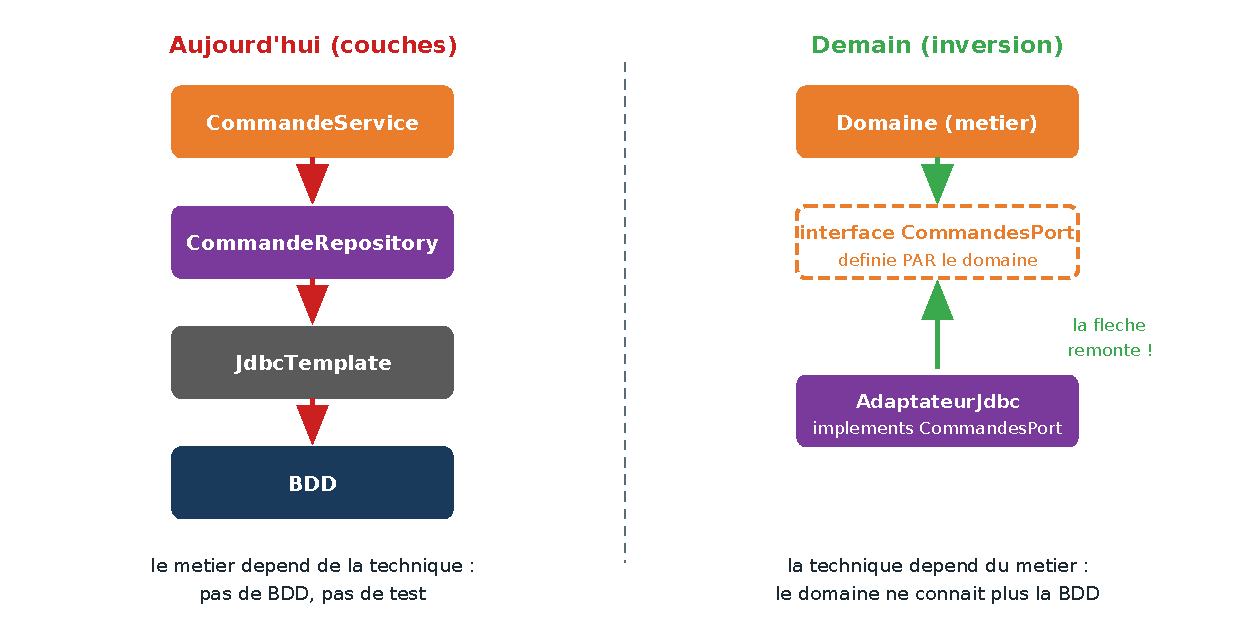
\includegraphics[width=0.55\linewidth]{figC_inversion}
\end{frame}

\begin{frame}{La question qui change tout}
\begin{ucadpiege}[Qui possède l'interface ?]
{\small Une interface ne suffit pas à inverser quoi que ce soit : si \texttt{CommandeRepository} définit lui-même son interface dans le paquetage \texttt{repository}, le domaine qui l'importe dépend \emph{toujours} de la persistance. L'inversion se joue sur la \textbf{propriété} : l'interface habite \textbf{chez le domaine}, écrite dans \textbf{son} vocabulaire.}
\end{ucadpiege}
\begin{itemize}\small
  \item Le domaine déclare : \emph{« j'ai besoin qu'on me sauvegarde des commandes »} — il écrit \texttt{CommandesPort} chez lui.
  \item La technique répond : \emph{« je sais faire, en JDBC »} — l'adaptateur \textbf{implémente} le port, et c'est donc \emph{lui} qui importe le domaine. La flèche a remonté.
\end{itemize}
\begin{ucadret}[À retenir]
{\small Inverser une dépendance, c'est déplacer la \textbf{propriété du contrat} : le métier ne demande plus la permission à la technique — il publie ses exigences, la technique s'y plie.}
\end{ucadret}
\end{frame}

% #####################################################################
\section{Ports et adaptateurs}

\begin{frame}{L'architecture hexagonale}
\begin{ucaddef}[Définition (Alistair Cockburn, 2005)]
{\small L'architecture \textbf{hexagonale} (\emph{ports \& adaptateurs}) place le domaine au centre, entouré de \textbf{ports} — les interfaces qu'il définit. Les \textbf{adaptateurs} traduisent le monde extérieur vers les ports ou les implémentent. Règle unique : \textbf{toutes les dépendances pointent vers le centre}.}
\end{ucaddef}
\centering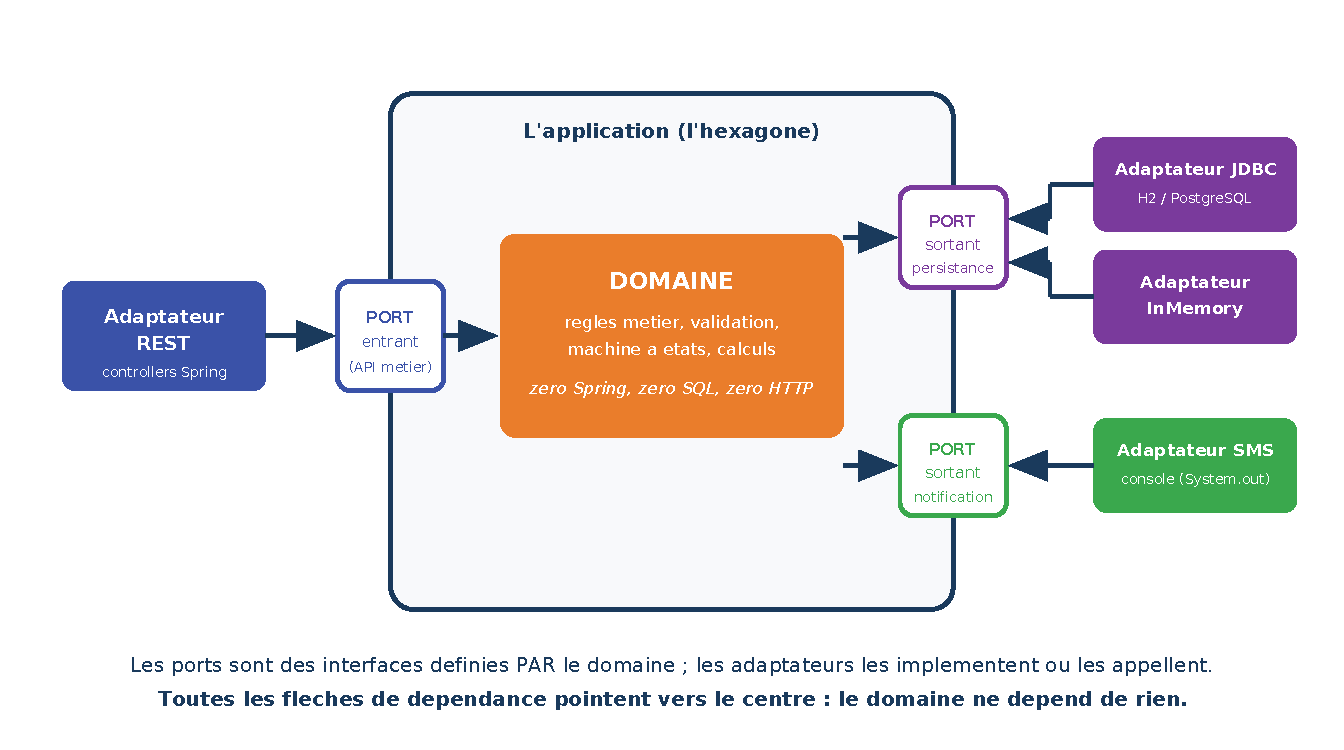
\includegraphics[width=0.50\linewidth]{figD_hexagone}
\end{frame}

\begin{frame}{Ports entrants, ports sortants}
{\small\begin{tabular}{p{0.20\linewidth}p{0.34\linewidth}p{0.34\linewidth}}
\toprule
 & \textbf{Port entrant} & \textbf{Port sortant}\\
\midrule
Qui l'appelle ? & le monde extérieur (REST, plus tard : messages) & le domaine\\
\addlinespace
Qui l'implémente ? & le domaine & un adaptateur technique (JDBC, SMS...)\\
\addlinespace
Chez SénResto & \emph{« créer une commande, la confirmer... »} & \emph{« sauvegarder, chercher un livreur, notifier »}\\
\bottomrule
\end{tabular}}
\vskip4pt
\begin{ucadex}[Le test du vocabulaire]
{\small Lisez un port à voix haute : s'il parle de \texttt{SELECT}, de JSON ou de HTTP, il est mal placé. \texttt{CommandesPort.sauvegarder(commande)} — du métier. \texttt{executerRequete(sql)} — de la technique déguisée.}
\end{ucadex}
\end{frame}

\begin{frame}[fragile]{À quoi ressemble un port}
{\small Le domaine écrit son besoin, dans son vocabulaire, chez lui :}
\begin{lstlisting}
package sn.ucad.senresto.domaine.port;

/** Ce dont le metier des commandes a besoin — rien de plus. */
public interface LivreursPort {
    Optional<Livreur> premierDisponible();
    void reserver(long livreurId);
    void liberer(long livreurId);
}
\end{lstlisting}
\begin{itemize}\small
  \item Aucune annotation Spring, aucun mot technique : ce fichier compilerait en 2005 comme en 2035.
  \item L'adaptateur JDBC du Lab 1 devient : \texttt{class AdaptateurLivreursJdbc implements LivreursPort} — trois méthodes déjà écrites, seule l'\emph{appartenance} change.
\end{itemize}
\begin{ucadret}[À retenir]
{\small Au Lab 2, vous n'écrirez presque pas de code nouveau : vous déplacerez la \textbf{propriété} du code existant. C'est un refactoring de frontières, pas une réécriture.}
\end{ucadret}
\end{frame}

% #####################################################################
\section{Le swap, la preuve}

\begin{frame}{Le moment magique : changer la technique}
\centering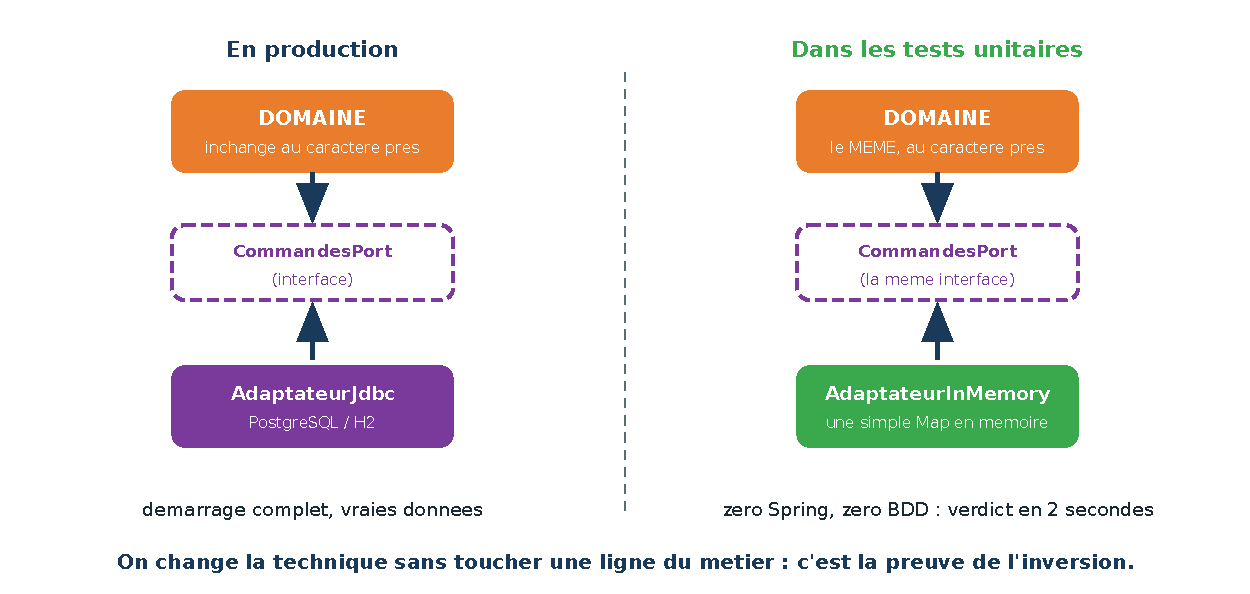
\includegraphics[width=0.64\linewidth]{figE_swap}
\end{frame}

\begin{frame}[fragile]{Le métier testé en deux secondes}
{\small L'adaptateur \emph{in-memory} — une Map — implémente les mêmes ports. Le test unitaire devient trivial :}
\begin{lstlisting}
@Test
void lesFraisDeLivraisonSuiventLeQuartier() {
    var domaine = new CommandeMetier(new CommandesEnMemoire(),
            new RestaurantsEnMemoire(), new LivreursEnMemoire(),
            new NotificationsEnMemoire());
    var commande = domaine.creer(new CommandeRequete(
            "Awa Ba", "771112233", "Ouakam", 1L, 2));
    assertEquals(2500 * 2 + 1500, commande.montantTotal()); // verdict : ~2 s
}
\end{lstlisting}
\begin{itemize}\small
  \item Zéro Spring, zéro BDD, zéro HTTP : on instancie le domaine \textbf{au constructeur}, comme n'importe quel objet Java.
  \item Les 4 tests d'intégration restent en poste : ils vérifient le \emph{branchement} complet. Les deux familles de tests sont complémentaires — rapides et nombreux au centre, lents et rares en périphérie.
\end{itemize}
\end{frame}

\begin{frame}{Ce que l'hexagone achète — et ce qu'il coûte}
\begin{itemize}\small
  \item \textbf{Achète} : le métier testable au centre ; la BDD, le framework, le canal de notification remplaçables sans toucher au domaine ; et une frontière prête pour la suite — au Lab 4, \emph{extraire} un module sera d'autant plus simple que ses dépendances passent déjà par des ports.
  \item \textbf{Coûte} : des interfaces en plus, une indirection en plus, une discipline de vocabulaire permanente. Pour un script jetable, ce serait du zèle ; pour un système qui doit vivre et évoluer, c'est un investissement.
\end{itemize}
\begin{ucadret}[À retenir — le réflexe de l'architecte]
{\small Toujours la même question : \emph{qu'est-ce que j'achète, avec quoi je le paie ?} Votre ADR n\textsuperscript{o}2 devra répondre pour SénResto — pas en général.}
\end{ucadret}
\end{frame}

% #####################################################################
\section{Le lab}

\begin{frame}{Le chemin du Lab 2}
\centering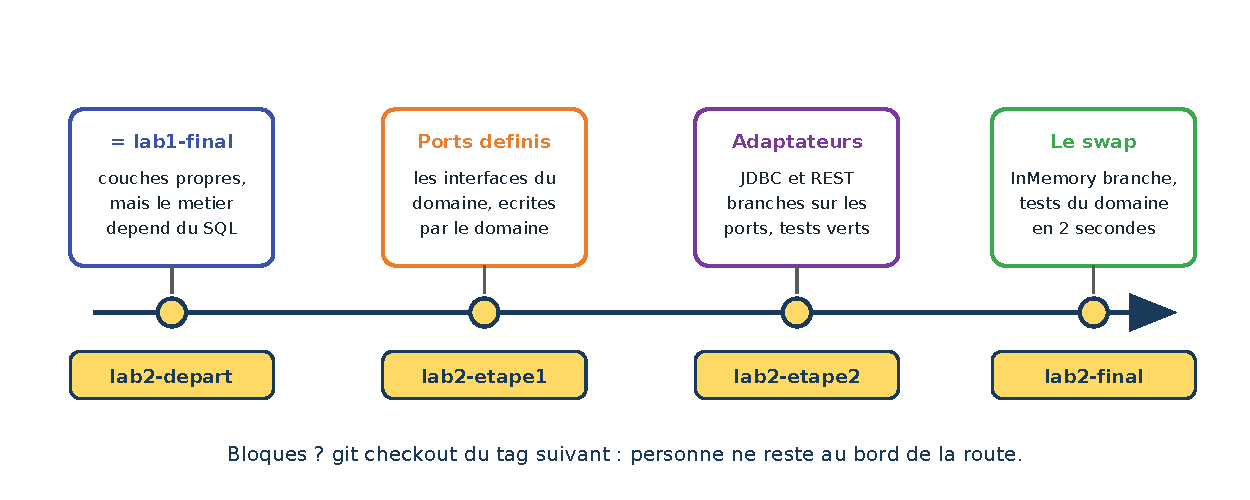
\includegraphics[width=0.80\linewidth]{figF_chemin_lab2}

{\scriptsize Point de départ : votre \texttt{lab1-final}. Le comportement de l'API ne change pas d'un octet — les 4 tests d'intégration restent les juges de paix.}
\end{frame}

\begin{frame}{Votre mission d'aujourd'hui}
{\scriptsize\begin{tabular}{p{0.20\linewidth}p{0.72\linewidth}}
\toprule
\textbf{Rôle} & \textbf{Pilotage au Lab 2}\\
\midrule
Le Doyen & branches, merges, tags — et l'ADR avec l'Architecte du jour\\
L'Huissier & le domaine des commandes : \texttt{CommandeMetier} + ports sortants\\
Le Rédacteur & l'adaptateur REST (controllers) branché sur les ports entrants\\
Le Notaire & les adaptateurs JDBC : \texttt{implements} des ports, SQL inchangé\\
L'Appariteur & les adaptateurs in-memory + les nouveaux tests unitaires du domaine\\
\bottomrule
\end{tabular}}
\vskip4pt
\begin{ucadrec}[Le livrable individuel de la séance]
{\small L'\textbf{Architecte du jour} signe l'\textbf{ADR n\textsuperscript{o}2 : « Pourquoi inverser les dépendances ? »} — une page, deux alternatives sérieuses, deux conséquences négatives assumées.}
\end{ucadrec}
\end{frame}

\begin{frame}{L'essentiel de la séance}
\begin{ucadret}[À retenir]
{\footnotesize
\begin{itemize}
  \item Des couches propres ne suffisent pas : tant que les flèches descendent vers la technique, \textbf{le métier reste prisonnier}.
  \item L'inversion se joue sur la \textbf{propriété de l'interface} : le port appartient au domaine, écrit dans son vocabulaire.
  \item \textbf{Hexagone} = domaine au centre, ports à la frontière, adaptateurs autour — toutes les dépendances pointent vers le centre.
  \item La preuve par le \textbf{swap} : même domaine, adaptateur JDBC en production, Map en mémoire dans les tests — verdict en 2 secondes.
\end{itemize}}
\end{ucadret}
\begin{ucadfront}[La question qui ouvre la séance 3]
{\footnotesize Votre hexagone protège le métier... mais tout SénResto vit dans \emph{un seul} hexagone : Catalogue, Commandes, Paiement, Livraison s'y mélangent. Où sont les frontières \emph{entre les métiers} ? Réponse au Lab 3 : le monolithe modulaire.}
\end{ucadfront}
\end{frame}

\end{document}
